\documentclass[11pt, a4paper]{article} 
\usepackage{babel}
\usepackage{booktabs}
\usepackage{comment} 
\usepackage[utf8]{inputenc} % odpowiednie kodowanie znaków
\usepackage[T1, T2A]{fontenc} 
\usepackage{graphicx} %wstawianie obrazków
\usepackage{float} %ustawianie obraków/tabel
\usepackage{multirow}
\usepackage{amsmath, amsfonts,amsthm} 
\usepackage{amsthm} %do twierdzen itd
\usepackage{mathtools}
\usepackage{blindtext} 
\usepackage{geometry}
\usepackage{graphicx}
\usepackage{amssymb}
\usepackage{tikz-cd}
\usepackage{lscape}
\usepackage{hyperref}
\usepackage{XCharter}
\usepackage{dsfont}
\usepackage[labelfont=bf]{caption}
\usepackage{caption}
\usepackage{subcaption}
\usepackage{pbox}
\usepackage{tikz}
\usepackage{tikz-feynman}

\setlength{\parindent}{15pt} 

%%%%%%%%%%%%%%%%%%%%%%%%

\title{\vspace{-2cm}On the Landau pole in quantum electrodynamics and the possible quantum gravity corrections}
\author{{Wojciech Śmiałek}\\
\\
{\textit{Supervisor}} \\
{Jan Kwapisz phd.}}
\date{}

\begin{document}
\maketitle

\section*{Introduction}

\section{Standard model etc.}
The Standard Model of particle physics is a unified description of all quantum fields observed in physics. 
It strives to predict all the phenomena observed at microscopic scales while maintaining theoretical
self-consistency and certain mathematical aesthetics. The predictive power of Standard Model, with its most
famous examples like precision tests of electron anomalous magnetic moment or the existence of Higgs' boson,
makes it ungrounded to postulate a fundamental physical theory that would not reduce to SM in the suitable limit, at least
as an effective field theory.
Standard Model, however, certainly is not a complete theory of physical reality, as it does not include a description
of gravity. Above the Planck scale $E_p \approx 10^{19} \ \text{GeV}$ quantum effects of gravity are expected to dominate
and predictions of both the SM and Einstein's theory of gravity are not expected to apply.
One should not be surprised, if at scales above $E_p$ Standard Model exhibits internal inconsistencies.
Given the requirements of compatibility with SM and predictivity (above the Planck scale), a good criterion/test
for any theory of quantum gravity should be for it to resolve the problems that arise in SM due to absence of
gravitational interaction. 
One of the big issues of the SM is the quantum triviality problem for the electroweak $U(1)$ gauge coupling and
the scalar higgs boson quartic coupling.
In the pure electroweak theory, one loop $\beta$-function of the abelian gauge \cite{betaf scalar} \cite{betaf chiral lagrangian} is:% Ref higgs paper instead
\begin{equation}
    \beta_{g_Y} = \beta_{g_Y}^{(3)} g_Y^3 = \frac{41}{6} \frac{g_Y^3}{16 \pi^2}
\end{equation}
This predicts a running of gauge coupling that would diverge at a momentum scale $\mu = \left(2 g_{Y\text{obs}}^2 \ \beta_{g_Y}^{(3)} \right)^{-1} $.
Conversely, taking any arbitrarily high value of the bare coupling, the only possible value of $g_{Y\text{obs}}$ should be 0, making
the theory trivial, i.e. non-interacting.
% In analogy to the QED fine structure constant, we define a dimensionless abelian gauge paramter as $\alpha_Y = g_Y^2 / 4 \pi$.
% It is related to the ordinary $\alpha_\text{QED}$ by a Weinberg angle and its value is known very precisely
% \begin{equation}
%     \alpha_Y = \frac{\alpha_\text{QED}}{\cos^2 \theta_W} = 0.0093905(30) % Two references to alpha and th_w, ogarnąć propagację niepewności
% \end{equation}
\begin{figure}[H]
    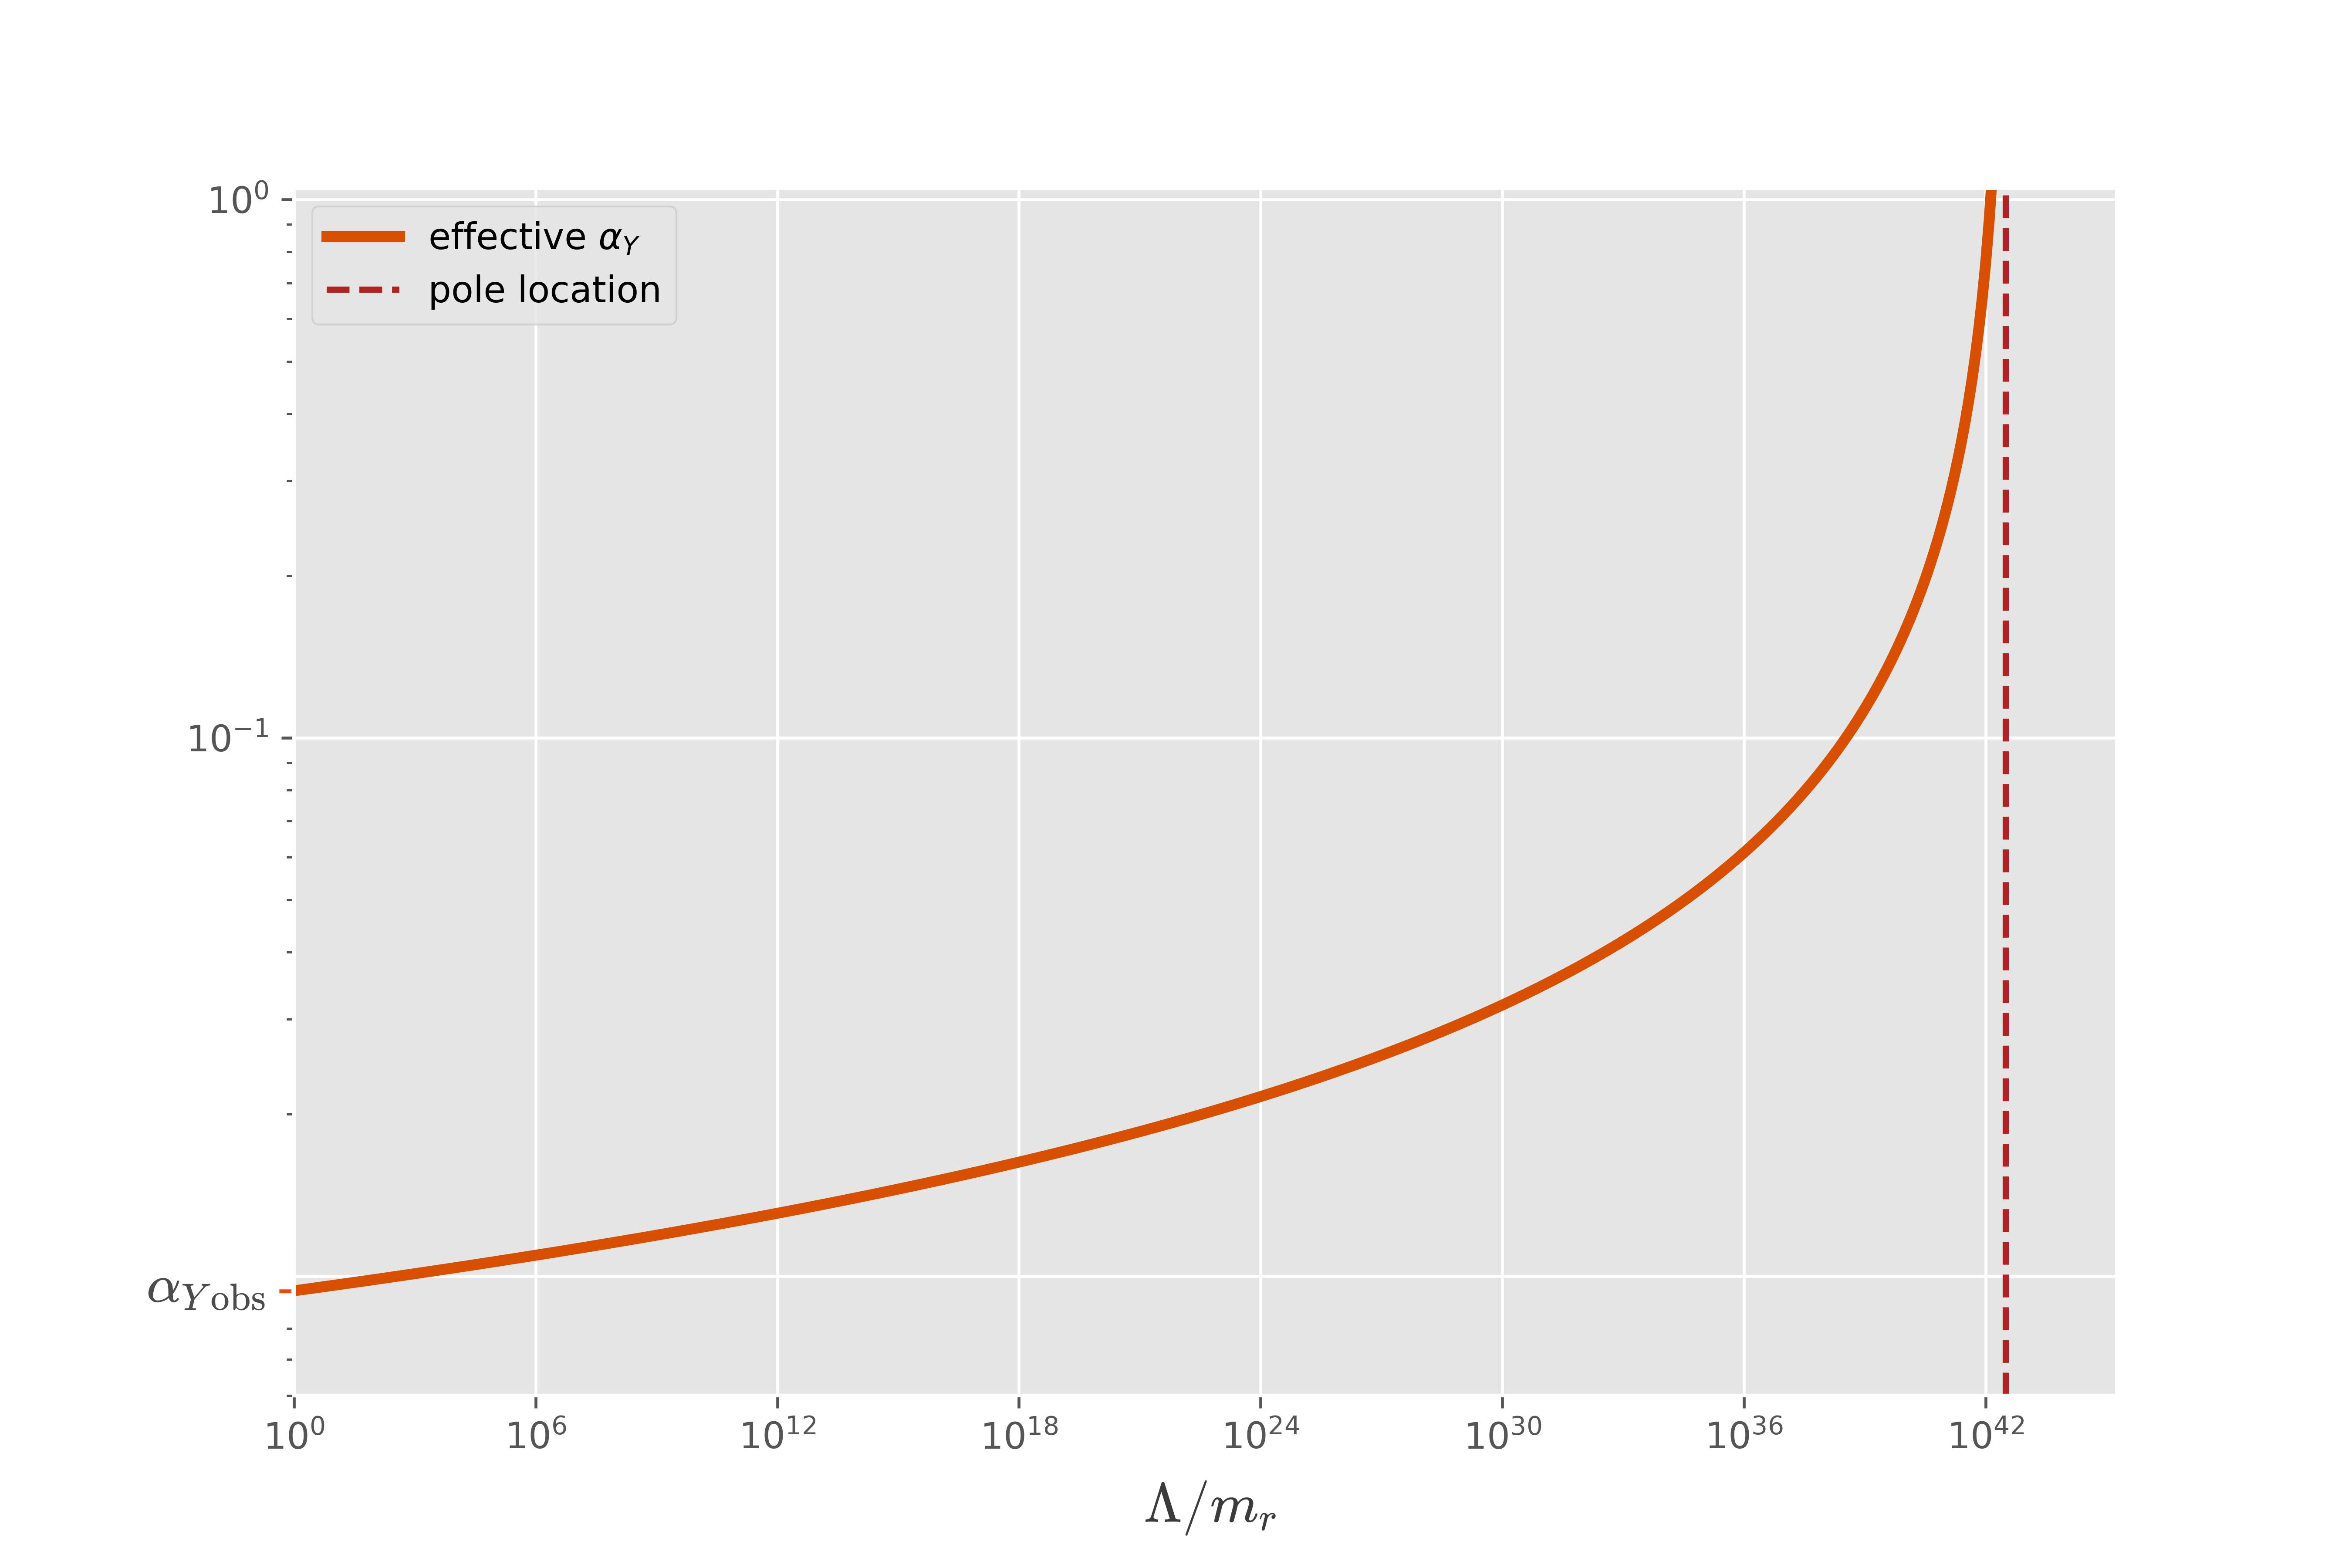
\includegraphics[width=1\textwidth]{../plotr.jpg}
    \caption{Running of the abelian gauge parameter $\alpha_Y = \frac{g_Y^2}{4\pi}$. Observed value $\alpha_{Y\text{obs}}$ is taken from [refs]. 
    Landau Pole marked at $\mu \approx 10^{42.5}$}
    \label{boxes}
\end{figure} 
Taking an electron mass as a reference scale, the location of abelian coupling landau pole will be of order $\Lambda \sim 10^{48} \ \text{eV}$, well above the Planck scale.

Similarly, quartic self-interaction of higgs field ...
(I tutaj napisać jak AS to rozwiązało i przewidziało masę higgsa więc dobry trop i wogle)
% I dopisać że do przewidzenia masy higgsa potrzeba żeby wkład od grawitacji do U(1) był ujemny, co my tutaj pokazujemy

% For the abelian gauge coupling $g$ with vanishing
% canonical dimension, the Ward-Takahashi identities imply a relation between the $\beta$-function of the coupling and the anomalous
% dimension $\eta_A$ of the gauge field. In the pure electroweak theory 
% Landau Pole
% Landau Pole for abelian hypercharge - figure
% + AS resolution of higgs triviality

% Ogólnie problemy SM
% Grand unification vs brak rozpadu protonu i prospects
% Alternatywa dla potrzeby gut - częścią tego istnienie fixed point of abelian coupling przy dodaniu grawitacji

\section{Discussion of literature etc.}

As the Landau Pole of abelian coupling is situated well above the Planck scale, one can conjecture that
its existence is due to the abence of quantum gravitational effects in the theory.
Even without postulating a UV-complete gravitational theory, it is beneficial to investigate
the impact of graviton on the running of abelian coupling [Wilczek ... czy coś]


% QED is a perturbatively renormalizable theory, i.e. it allows to calculate probability amplitudes for physical processes
% up to an arbitrary order in couplings.
%% One loop beta function of qed
%% Discussion of landau pole
%% General form in the presence of quantum gravity
% Wilczek paper
%% Qualitative difference

\section{Obtained results etc.}


\subsection{The Functional Renormalization Group Equation}

\subsubsection*{\centering Effective action}

In the traditional Wilsonian approach to renormalization, a single step of renormalization procedure consists of
a functional integration of high-momentum fluctuations, followed by a rescaling of physical lengths and momenta, and
renormalization of fields. All of this leaves the non-perturbed theory unchanged, affecting only the couplings.
Before the rescaling and renormalization operations [we are dealing with] the so-called Wilsonian effective action ($S_{\text{eff}}$).
It describes the behaviour of fields for the processes below certain energy scale $b\Lambda$, lower than the original cutoff $\Lambda$.
$S_{\text{eff}}$ generally contains all operators with higer dimensions in fields and derivatives.
These corrections (...) but they allow us to neglect field modes larger than $\mu = b\Lambda$ and deal only with non-divergent diagrams.
The argument of $S_{\text{eff}}$ is still a quantum field, in the sense that the functional integral is performed over it. %It also,
% in some sense, loses information about the high-energy physics.

The object, that we will call an effective action $\Gamma$ is different and should not be confused with $S_{\text{eff}}$.
Let us start from the euclidean partition function for scalar field theory. The definition for other theories
come as a straight-forward generalization.
\begin{equation}
    Z[j] = \int \mathcal{D}\phi \ e^{-S[\phi] + \int dx j \phi}
\end{equation}
The generating functional of connected Green's functions is defined as
\begin{equation}
    W[j] = \log{Z[j]}
\end{equation}
The effective action functional is defined using the Legendre transformation of $W[j]$.
\begin{equation}
    \Gamma[\phi_c] = W[j_\phi] - \int d^4 x j_\phi(x) \phi(x)
\end{equation}
The two fields $\phi_c$ and $j_\phi$ are inverses of each other, defined as the solution to
\begin{equation}
    \phi_c(x) = \langle \hat\phi (x) \rangle_j = \frac{\delta W[j]}{\delta j(x)}
\end{equation}
The argument of the effective action is a classical field and there is no functional integral to be performed over it.
Rather, in $\Gamma$ all of the fluctuations are integrated out, but only one-particle irreducible diagrams
are included. $\Gamma$ acts as a generating functional of 1PI Green's functions. Extremizing effective, rather than
the clasical action, yields the equations of motion for vacuum expectation values of the quantum fields.

In its bare form, effective action is ill-defined, as was expected. One option is to introduce a UV cutoff $\Lambda$
and study the rg flow through divergences proportional to $\Lambda$. The modification we will employ, however, involves
an IR cutoff inserted through adding a regulator term $\Delta S_k[\phi]$ to the bare action $S[\phi]$ in the definition of partition function
and subtracted from the final form of effective action. Explicitly, this new object, called the effective average action (EAA) is defined as
\begin{gather}
    W_k[j] = \log{\int \mathcal{D}\phi \ e^{-S[\phi] - \Delta S_k[\phi] + \int dx j \phi}}\\
    \Gamma_k[\phi_c] = W_k[j_\phi] - \int d^4 x j_\phi(x) \phi(x) - \Delta S_k[\phi]
\end{gather}
Motivation for introducing EAA will become clear when we study the functional renormalization group

\subsubsection*{\centering Infrared regulator and the scheme dependence}

\subsubsection*{\centering Beta functional and the functional renormalization group}

The $\Gamma_k$ is IR-regulated, but still it is ill-defined, because of the UV divergences. 
However, in studying the scale dependence of couplings we will not use full EAA, 
but its derivative with respect to $t = \log{k}$.
We assume the theory space in which $\Gamma_k$ takes the form
\begin{equation}
    \Gamma_k = \sum_i g_i(k) \ \mathcal{O}_i [\phi]
\end{equation}
Where $\mathcal{O}_i (\phi)$ are integrals of monomials of fields or positive powers of field derivatives 
and $g_i(k)$ are scale-dependent couplings.
The coefficients in EAA derivative with respect to $t$ are therefore simply the beta functions of corresponding operators
\begin{equation}
    \frac{d \Gamma_k}{dt} = \sum_i \frac{d g_i}{dt} \ \mathcal{O}_i [\phi] = \beta_i(g,k) \ \mathcal{O}_i [\phi]
\end{equation}
The beta functions may depend on all the couplings, as well as the renormalization scale $k$.
They can be extracted from $\frac{d \Gamma_k}{dt}$ via a suitable projection operator. 
The $\frac{d \Gamma_k}{dt}$ is called the beta functional. This functional, as can be shown, is finite[refs].
This is because the beta functional can be viewed as a difference between effective actions with infinitesimally
different cutoffs. The UV divergences in the difference will cancel, and what remains is the finite rest
dependent on the degrees of freedom with momenta close to the renormalization scale.

Let us calculate the derivatives of $W_k$ and $\Delta S_k$ with respect to $t$
\begin{gather}
    \frac{d W_k}{dt} = \frac{d}{dt}\log{Z_k} = - \frac{1}{Z_k} \int \mathcal{D}\phi \ e^{-S[\phi] - \Delta S_k[\phi] + \int dx j \phi}  \cdot \frac{d \Delta S_k}{dt} \\
    \frac{d \Delta S_k}{dt} = \frac{1}{2} \int d^4 x \ \phi \ \frac{d R_k}{dt} \ \phi
\end{gather}
This lets us write
\begin{equation}
    \frac{d \Gamma_k}{dt} = \frac{d \langle \Delta S_k \rangle}{dt} - \frac{d \Delta S_k }{dt} = \frac{1}{2} \operatorname{Tr} \left[ (\langle\phi\phi\rangle - \langle\phi\rangle^2) \cdot \frac{d R_k}{dt} \right]
\end{equation}
Where $\operatorname{Tr}$ denotes ... and the $\langle\cdots\rangle$ - ...
The expression $(\langle\phi\phi\rangle - \langle\phi\rangle^2)$ can be shown to be equal to $\frac{\delta^2 W_k}{\delta j \delta j}$ [cite]
From there, if we would express $\frac{\delta^2 W_k}{\delta j \delta j}$ in terms of $\Gamma_k$, we could
write an exact, first order differential equation for the effective average action.
In fact, the relationship between (them) is very simple. Recall, that $\Gamma_k + \Delta S_k$ is a Legendre transform of $W_k$. For any
two functions $f$ and $g$, one being the Legendre transform of the other, we have $f'' = (g'')^{-1}$. This remains true for the functional derivation.
Using this information and immediatly performing field derivative over $\Delta S_k$, we can write the equation for $\Gamma_k$:
\begin{equation}
    \frac{d \Gamma_k}{dt} = \frac{1}{2} \operatorname{Tr} \left[ \left(\frac{\delta^2 \Gamma_k}{\delta \phi \delta \phi} + R_k\right)^{-1} \cdot \frac{d R_k}{dt} \right]
    \label{FRGE}
\end{equation}
This is the functional renormalization group equation (FRGE) or the Wetterich equation. (...)
In its original form, FRGE is not well suited for performing specific calculations. One very intuitive method, which
we will use is the $\mathcal{PF}$-expansion, that allows us to use the Feynman diagrams for calculating the RHS of equation (\ref{FRGE})
up to the desired order in couplings. The term inside the trace including Second derivative of EAA
will in general be, for spinor or tensor fields, a functional hessian matrix. We can decompose this term into a
regulated inverse propagator matrix $\mathcal{P}$ and a rest, which will include the derivatives of terms non quadratic in fields.
\begin{equation}
    \frac{\delta^2 \Gamma_k}{\delta \phi \delta \phi} + R_k = \mathcal{P} + \mathcal{F}
\end{equation}
First, let us notice that the entire expression inside trace can be expressed as a $\log{(\mathcal{P}+\mathcal{F})}$, upon which acts
a $t$-derivative sensitive only on the $t$ dependence in $R_k$. Explicitly, we can write:
\begin{equation}
    \left(\mathcal{P} + \mathcal{F}\right)^{-1} \cdot \partial_t R_k = \left(\mathcal{P} + \mathcal{F}\right)^{-1} \cdot \widetilde{\partial_t} \left(\mathcal{P}+\mathcal{F}\right) = \widetilde{\partial_t} \log{\left(\mathcal{P}+\mathcal{F}\right)}; \quad \widetilde{\partial_t} = \int \partial_t R_k \frac{\delta}{\delta R_k}
\end{equation}
Now, we can recall the series expansion of $\log{(1+x)}$ around $x=0$ and after some simple manipulations, obtain an expansion of functional trace in (\ref{FRGE}) in
the number of $\mathcal{F}$-terms
\begin{gather}
    \frac{d \Gamma_k}{dt} = \frac{1}{2} \operatorname{Tr} \left[ \widetilde{\partial_t} \log{\left(\mathcal{P}+\mathcal{F}\right)} \right] = \frac{1}{2} \operatorname{Tr} \left[ \widetilde{\partial_t} \left(\log{\mathcal{P}} + \log{(1+\mathcal{P}^{-1}\mathcal{F})}\right) \right] \\ =  \frac{1}{2} \operatorname{Tr} \left[ \widetilde{\partial_t} \log{\mathcal{P}} \right] + \frac{1}{2} \sum_{n=1}^{\infty} \frac{(-1)^{n-1}}{n} \operatorname{Tr}\left[\widetilde{\partial_t}\left(\mathcal{P}^{-1}\mathcal{F}\right)^n\right]
\end{gather}

\subsection{xx}

A great advantage of functional renormalization group is that in principle, if all terms
allowed by the symmetries are included in the effective action, one obtains a set of first order
differential equations that contain full information about the RG flow in the theory, without referring to the perturbative methods.
In practice, that would mean dealing with infinitely many differential equations. The only way
to extract actual predictions from the FRGE is to truncate effective action to a finite number
of terms. If beta functions computed in given truncation changes little after adding higher terms to the EA,
it is a good argument for considering the truncation a good approximation of the full theory. (...)
\begin{gather}
    \mathcal{L} = \mathcal{L}_{EH} + \mathcal{L}_A + \mathcal{L}_{GGF} + \mathcal{L}_{AGF} \\
    \mathcal{L}_{EH} = \sqrt{\mathbf{g}} \ \frac{k^2}{\kappa} \left( k^2 \Lambda - R\right) \\
    \mathcal{L}_A = \sqrt{\mathbf{g}} \ Z_A \frac{1}{4} F^{\mu\nu} F_{\mu\nu} \\
    \mathcal{L}_{AGF} = \sqrt{\mathbf{g}} \ Z_A \frac{1}{2 \alpha_A} \left( \partial_\mu A^\mu \ \partial_\nu A^\nu \right) \\
    \mathcal{L}_{GGF} = \sqrt{\mathbf{g}} \ Z_h \frac{1}{32 \pi \alpha_h} \left(\partial_\mu h^{\mu\nu} - \frac{1+\beta_h}{4} \partial^\nu h^\rho_{\; \rho} \right)^2\\
\end{gather}
\begin{equation}
    \Gamma[\mathbf{\Phi}] = \int d^4 x \ \mathcal{L} + w_2 (F^{\mu\nu} F_{\mu\nu})^2
\end{equation}
%% Describe action and truncation
Beta functions extracted from the full EA cannot depend on the choice of gauge parameters.
Introducing truncations, however, means that gauge dependence may not cancel entirely (...).
%% ?? Że będziemy sprawdzać zależność od gauge parameter ??
Another in principle redundant choice is a form of the regulator. For two different regulators,
$\Gamma_k$ will include field modes weighted in a different manner, so this choice simply
sets the definition of the object $\Gamma_k$. 
This means, that beta functions computed with different regulators will differ, but
if the regulator is picked in such way that it executes a proper IR cutoff,
it will always give the same results in the physical limit $k \rightarrow 0$. There should also be no
qualitative differences in the behaviour of RG flow depending on the regulators.
%% Coś o tym że to będziemy tu sprawdzać


\section*{Summary}

\begin{thebibliography}{9}
    \bibitem{betaf scalar}
    Brod, J., Polonsky, Z. Two-loop beta function for complex scalar electroweak multiplets. J. High Energ. Phys. 2020, 158 (2020). https://doi.org/10.1007/JHEP09(2020)158
    \bibitem{betaf chiral lagrangian}
    Buchalla, G., Catà, O., Celis, A., Knecht, M., Krause, C., Complete one-loop renormalization of the Higgs-electroweak chiral Lagrangian. Nuclear Phys. B 2018, 928 (93). https://doi.org/10.1016/j.nuclphysb.2018.01.009
\end{thebibliography}

\end{document}